\section{Application}
\label{sec:app}
 The segmentation results are further used to 3D building reconstruction. We make use of the depth map and generate the point cloud of remote sensing images. After that, the 3D building reconstruction methods could applied to the generated point cloud. In this paper, the approach proposed by zhou\cite{IEEEexample:zhou20112} are used to generate the 3D models of buildings in the scene. Fig.~\ref{fig:Vaihingen-3Dmodeling}
and Fig.~\ref{fig:Potsdam-3Dmodeling} show the 3D models of Vaihingen and Potsdam dataset respectively. The details of a single building are also presented. From the figures, we can see the 3D models preserve the characteristics of buildings well whether the structure of the roof or the simplification of details.
\begin{figure}
\centering
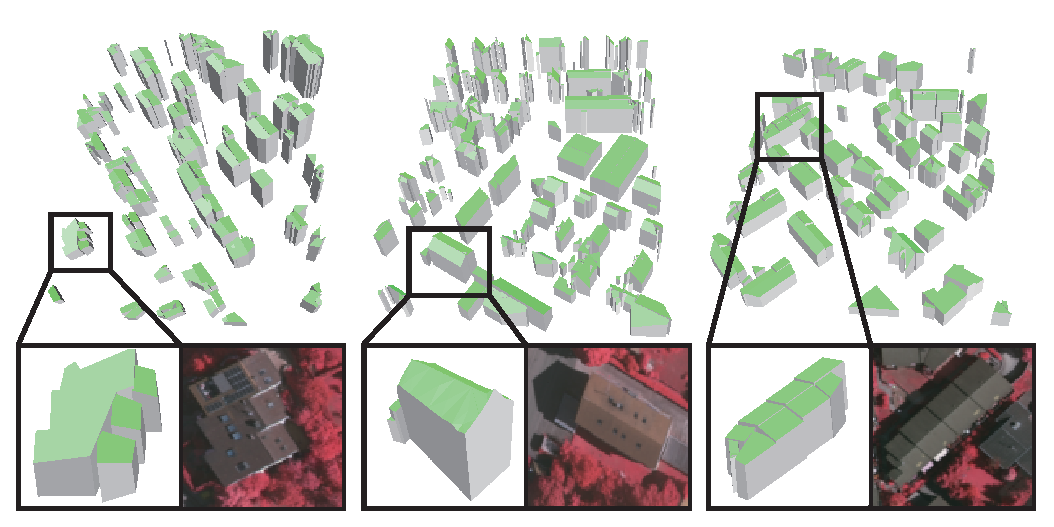
\includegraphics[width=8.7cm]{Figures/Vaihigen_3Dmodelling.eps}
\caption{The 3D modelling of Veihingen dataset. The single building model and its corresponding optical patch were shown together.}
\label{fig:Vaihingen-3Dmodeling}
\end{figure}

\begin{figure}
\centering
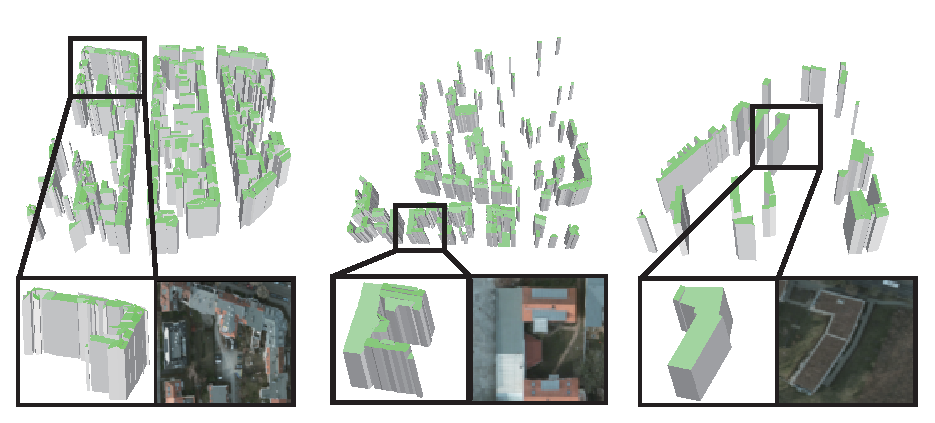
\includegraphics[width=8.7cm]{Figures/potsdam_models.eps}
\caption{The 3D modelling of Potsdam dataset. The single building model and its corresponding optical patch were shown together.}
\label{fig:Potsdam-3Dmodeling}
\end{figure}
